\documentclass[11pt]{article}
\setlength{\topmargin}{-.5in}
\setlength{\textheight}{23.5cm}
\setlength{\textwidth}{17.0cm}
\setlength{\oddsidemargin}{.025in}
\setlength{\evensidemargin}{.025in}
\setlength{\textwidth}{6.25in}
\usepackage{amsmath}
\usepackage{graphicx}
\usepackage{verbatim}   % useful for program listings
\usepackage{color}      % use if color is used in text
\usepackage{subfigure}  % use for side-by-side figures
\begin{document}
\begin{titlepage}
\begin{center}
\textsc{ \LARGE Expanding QTL analysis \\}
\textsc{High performance computing of QTLs for experimental crosses\\}
\end{center}
$ $\\
\\\\\\\\\\\\\\\\
\\\\\\\\\\\\\\\\
\\\\\\\\\\\\\\\\
\\\\\\\\\\\\\\\\
\\\\\\\\\\\\\\\\
\begin{minipage}{0.5\textwidth}
  \begin{flushleft} \large
  \emph{Author:}\\
  Danny \textsc{Arends}\\
  $ $\\
  $ $\\
  \end{flushleft}
  \end{minipage}
  \begin{minipage}{0.5\textwidth}
  \begin{flushright} \large
  \emph{Supervision:} \\
  Dr. Pjotr \textsc{Prins}\\
  Dr. Ritsert \textsc{Jansen}\\
  Dr. Karl \textsc{Broman}\\
  \end{flushright}
\end{minipage}

\end{titlepage}
\input{Abstract.tex}
\newpage
\section*{Terms \& Abbreviations}
\begin{itemize}
	\item API - Application programming interface 
	\item AIC - Akaike's information criterion
	\item BC - Backcross (Specialized animal breeding technique)
  \item (M)Bp - (Mega)Basepair
	\item CIM - Composite interval mapping
	\item cM - centiMorgan
  \item CPU - Central processing unit
  \item Core - A single processing unit on a CPU
	\item F2 - F2 intercross (Specialized animal breeding technique)
  \item GPU - Graphics processing unit
  \item GWAS - Genomewide association study
	\item HPC(/V) - High performance computing (and visualisation)
	\item LCMS - Liquid chromatography-mass spectrometry
	\item LOD - -10Log(Pvalue) so a lod score of 3 means a chance of a 1000 : 1
  \item Molgenis - Molecular genetics information system
	\item MQM - Multiple QTL mapping \cite{jansen93}
	\item PBS - Portable Batch System \cite{PBS2000}
	\item QTL - Quantative Trait Locus
	\item eQTL - QTL associated with gene expression
	\item pQTL - QTL associated with protein abundance
	\item mQTL - QTL associated with metabolites
  \item R - Statistical programming language and environment
  \item R/qtl - R-package by Prof. K. Brohman
  \item RIL - Recombinant inbred line (Specialized animal breeding technique)
	\item RUG - University of Groningen
  \item SNOW - Simple Network of Workstations \cite{tierney04}
	\item XGAP - eXtensable Genotype And Phenotype dataplatform
\end{itemize}

\section{Introduction}
\subsection{r/qtl}
R/qtl is an open source package for mapping QTL in experimental crosses for the R programming language\cite{broman09}\cite{broman03}.
It can be used to analyse several types of experimental crosses (Backcross (BC), F2, Recombinant inbred lines (RIL), Intercrosses (IC)) 
. Furthermore it offers many methods for QTL mapping (Composite interval mapping (CIM), expectation maximization (EM), marker regression (MR) and 
Extended Haley-Knot (eHK)). Because R/qtl supports different experimental crosses and contains many extra functions (plotting, genotype checking, etc).
Because it is opensource software no cost are associated with usage of the R-package (or the R-software infrastructure). Also its opensource nature
 makes it easy for others to contribute to the package. 
Our goal is to make complex QTL mapping methods widely accessible and allow users to focus on modeling rather than computing. R/qtl 
is becoming an increasingly popular environment for QTL analysis and has its own stabile userbase\cite{broman03}.
\subsection{Molgenis \& XGAP}
Storing information is very important, it becomes even more crucial when large -omics datasets are involved. These -omics sets are ussually generated 
in plain text format and read into a database system (mySQL/Oracle/msSQL). However these systems are not tailored to the needs of this biological data.
Providing ussually only storage for the most basic of datatypes (integers,strings,etc), they ussually lack biological dataformats, but are very good 
at storing data within a strict format. The molgenis database system using the extensible genotype \& phenotype (XGAP) datamodel aims to solve both these problem.
It does so by providing an easy to change datamodel (XGAP), with a generator to change the currentdatabase layout with a push of the button. The adaptability
of the system allows for easy managment of constantly changing biological data. This is furthermore enhanched by allowing for 3th party plugin to be 
connected to the database system. Molgenis was used in our project as out dataproviding software and a plugin was designed and implemented to enable 
molgenis users to perform R/QTL analysis from a webenviroment.
\subsection{High Performance Computing (HPC)}
The university of Groningen has an institute dedicated to high performance computing. The cluster is comprised of 168 machines running on a dualcore CPU. To 
facilitate high performance computations a PBS\cite{PBS2000} jobsceduler is present on the cluster, together with an installation of R-2.9.0. When computational job become too big for a desktop computer, these HPC facilities can be used. 
Another part of the project was focused on using the high speed computing facilities available in combination with the molgenis database system. 
\newpage
\section{Materials}
\subsection{Biological datasets}
Different datasets were used to benchmark analysis:
\begin{itemize}
\item	Simulated datasets generated by R/qtl. \cite{broman03}
\item	Arabidopsis - RIL population between the arabidopsis strains: Landsberg erecta and Capeverdian islands, phenotypes: gene-expression, protein- and metabolite abundance. \cite{keurtj}
\item	Oats - F2 cross of Kanota X Ogle Oat. \cite{Oats}
\item	Rats - Backcross of 250 individuals, phenotype: Bloodpressure. \cite{Hyper}
\item	Listeria - F2 cross of 250 individuals mouse, phenotype: Listeria monocytogenes infection in the mouse. \cite{Listeria}
\end{itemize}
\subsection{Programming tools/compilers}
Several tools were used to create an interface between R/qtl and the MQM algorithm. The tools used are summarized below:
All programs and scripts and plotting code used or created is available at request. It is also available at GBIC and the students personal repository http://www.github.com/DannyArends
\begin{table}[ht]
	\begin{tabular}{l  l}
Basic tools & Notepad++\\
	& Miktex\\
	& R-2.8.1 with R/qtl\\
	& GIT 1.8.6\\
MQM & RTools\\
	& Dev-C++\\
	& SNOW\\
	& Microsoft visual studio 2008\\
	& openMP\\
Molgenis & Eclips\\	
	& MySQL 6.0\\
	& Molgenis distro 3.3\\
	& xGAP distro 1.1\\
	& Java SDK\\
	\end{tabular}
	\label{tbl:tools}
\end{table}
\subsection{Cluster infrastructure}
To analyse QTL's directly from a Molgenis webenvironment, additional calculation power is needed to perform these intensive calculations. 
Because QTL calculation can take upto (or more than) 24 hours these calculations should be performed by a separate machine 
or even a parallel processing cluster. The plugin created for the Molgenis system uses an SHH tunnel to connect to a machine running a PBS job scheduler. Any machine using PBS to schedule jobs can in theory be used when the following prerequisites are met:
\begin{itemize}
\item Reachable by SHH connection using a login and password
\item installed PBS job scheduling system
\item R 2.7.0+
\item R Packages: RCurl, molgenis, R/qtl (optional: SNOW)
\end{itemize}
An example of the plugin can be found here:\\ http:$\backslash$$\backslash$gbic.target.rug.nl:8080$\backslash$xgap4clusterdemo$\backslash$\\
\section{Method}
\subsection{Speeding up QTL analysis}
Within the emerging field of -omics data analysis QTL analysis is becoming more and more computationaly intensive. To speed up multiple trait analysis a parallellization strategy 
using MPI was implemented. The SNOW package \cite{tierney04}, provides an message passing interface (MPI) implementation for R. Using SNOW  
we can distribute calculations in batches across available computing cores on a multicore machine. The only requirement is that calculations
can be performed independent of eachother (see figure 1).
\subsection{QTL permutation analysis}
Using a permutation approach it is possible to estimate thresholds for QTL significance. Because shuffling data gives us an estimate on how significant our results are. Permutation is performed by calculating 
new trait values for each individual based on the variation in the original trait (see figure 1,2,5). Permutation is performed by 
randomly redistributing (the original) traitvalues across individuals (each endophenotype value is redistributed only once per permutation). 
Both methods of obtaining thresholds for QTL significance are implemented into the new bootstrap function in R/qtl. 
After adding two bootstrap methods (permutation, parametric bootstrap) a parallel permutation approach was developed and implemented using SNOW.
\subsubsection*{Single trait permutation}
Parallel permutation analysis takes the same approach as multiple trait calculations using SNOW. In the case 
of single trait permutations at the beginning of each run the traitvalues are randomly redistributed 
over the indiviuals and analysis continues like a multitrait analysis. Using permutation we calculate new traitvalues for each individual
(based on a random number chosen for each individual, and the variance in the original endophenotype). This process is repeated a $> 10000$ times
to get maximum LOD scores in random traits. The distribution of these maximum LOD scores enables us to estimate a threshold 
above which we call QTL's significant. QTLs above this threshold are identified as significant. Also here analysis time increases linearly with the number of bootstraps / permutations performed. A parallellization strategy was adopted to speed up calculations.
\subsubsection*{Genome scan significance and FDR}
When scanning multiple traits for QTLs, when doing an -omics experiment single trait thresholds are not sufficient. As a solution to this multiple testing problem we could set more 
stringent thresholds using bonferroni correction or B/H correction to estimate real QTL effect and false QTL hotspots. However when doing this a lot of power is lost, 
because of the stringent threshold. To estimate a genomewide threshold it is more rewarding to do a full genome permutation, 
in which the correlation structures between traits are maintained.\cite{eQTL1} In each permutation genotypes are randomly distributed between indiviudals, 
trait values remain unchanged, and a full parallel multitrait mapping of QTLs is performed (Figure 3). From these results we can calculate False Discovery Rates (FDR) for a given LOD score, this enables us to estimate how many of the QTLs above a certain threshold 
are significant, and what cutoff gives the fewest number of false positives.
\subsection{Multiple QTL mapping}
An implementation of MQM was made by R.C. Jansen in the C-programming language. The original C-source code was adapted and implemented beind R to be used with more ease by biological users. This is facilitated because the R programming language is very intuitive for first time users and provides advanced toold for average and professional users.
\subsubsection*{Model selection}
Model selection is done by employing a backward elimination of possible co-factors. Model selection strategy (how many QTLs are underlying a trait) 
is done by setting markers as cofactors for QTL analysis. Each cofactor is analyzed sequentially. If the model fit with cofactor is significantly better than without it, the cofactor is kept in the final model. This difference in fit between two models is determined by the AIC. So a model with a lower AIC is prefered above a model with a high AIC. The cofactor is dropped if the model gets a significantly worse fit with the data. The co-factors remaining after analysis 
are used in the mapping phase of the MQM algorithm, where they will serve as covariates during mapping.
\subsubsection*{QTL mapping}
QTL mapping in MQM is almost similar to composite interval mapping (CIM). We start out explaining how CIM works and will then explain the difference between CIM and MQM.
When using CIM we divide a chromosome in equally spaced regions (e.g. each region is 5 Cm long) by inserting pseudomarkers. For all these pseudomarkers the most likely genotype per individual is calculated using statistical genetics.
 After calculation of the most likely genotypes CIM uses maximum likelihood or restricted maximum likelihood to calculate a LOD score at each of these pseudomarkers. This is done by using the most 
likely genotype at those pseudomarkers. MQM does essentially the same thing dividing up the chromosomes in equally spaced regiosn, using pseudomarkers. MQM also maps LOD scores to these pseudomarkers. 
However for each pseudomarker not the most likely genotype per individual is determined. But at each pseudomarker all possible genotype are calculated and their 
probability of occuring (based on neighbouring markers). These genotypes are then used (weighted with the probability of occuring) to calculated LOD scores at each pseudomarker during the mapping of the QTLs.
\subsection{Benchmarking}
\subsubsection*{Multitrait and parallellization}
Our approach to employ parallel permutations was benchmarked against a version running serial computations. This was done to obtain an estimate 
on how much improvement can be gained when using multiple core analysis compared to a single core analysis. A summary of the benchmarking can be found in the results 
section, and the raw data is supplied as a table in the "additional tables" section. (see Tables: \ref{tbl:tabel2} \& \ref{tbl:tabel3})
\subsubsection*{MQM}
Benchmarking of MQM was done to get an estimate of scalability of the algorithm. Benchmarking was performed using the R-programming language 
and a dualcore desktop pc. To test the scalability of the MQM algorithm we pertubated several parameters that also vary during normal research, such as: Populations type (BC, F2, RIL), number of individuals, number of markers, number of co-factors under consideration during the model selection phase.

\subsection{Datastructuring and storage}
In R we adopted the R/qtl cross object format, however when sharing results with others 
(publication, etc) this binary format is not useful. Here databases can help, storing huge amounts of data like publicly available 
and / or private datasets. Adding data to a database in a transaction based way ensures data consistency. 
Also database systems allow for third party software to store and retrieve data from the database directly or via
a supplied application programming interface (API). The XGAP \cite{morris07} (Xtensible Genotype and Phenotype) datamodel is used 
to format data in a homogenous matter when storing data into a molgenisDB. This XGAP format ensures data 
is extensible and consistent. The molgenisDB system ensures dataconsistency and -coherency, plus allowing easy 
access from R / JAVA / SOAP or by using HTML scripting.
\subsection{HPC of QTLs using molgenisplugin}
A plugin was created to enable users to use the R/qtl package from the molgenis webenvironment. To use this plugin another machine is required 
to distribute jobs and do QTL analysis. This was done to separate QTL calculation from normal server operations.
The clusterplugin was tested using public datasets that are available from previously performed QTL research. Users can use the HPC cluster 
of the State University of Groningen to do high performance QTL analysis.
Furthermore we created an overview of the current infrastructure needed for a functional plugin. This overview can be found in figure 8. 
\subsection{Visualizations}
We added some new visualizations to graphically explore the data. Visualization is important when doing complex analysis because 
it gives graphical handles which one can work with. The new plotting methods were developed as an extention on the original plotting methods in R/qtl.
We created new plotting methods for many endophenotypes analysis and bootstrap analysis, these plotting methods are based on a timeseries plotting 
routine made by R. Brouwer\cite{brouwer09}.
\section{Results}

\subsection{Datastructuring and storage}
Methods to connect R/qtl to XGAP/molgenisDB were writen in the R programming language using the molgenis R-API. 
To use the molgenis API for R an R-package named Rcurl \cite{Rcurl08} is used to make HTTP connections to the 
molgenis server.

\begin{figure}[ht]  
\centering
  \hfill
  \fbox{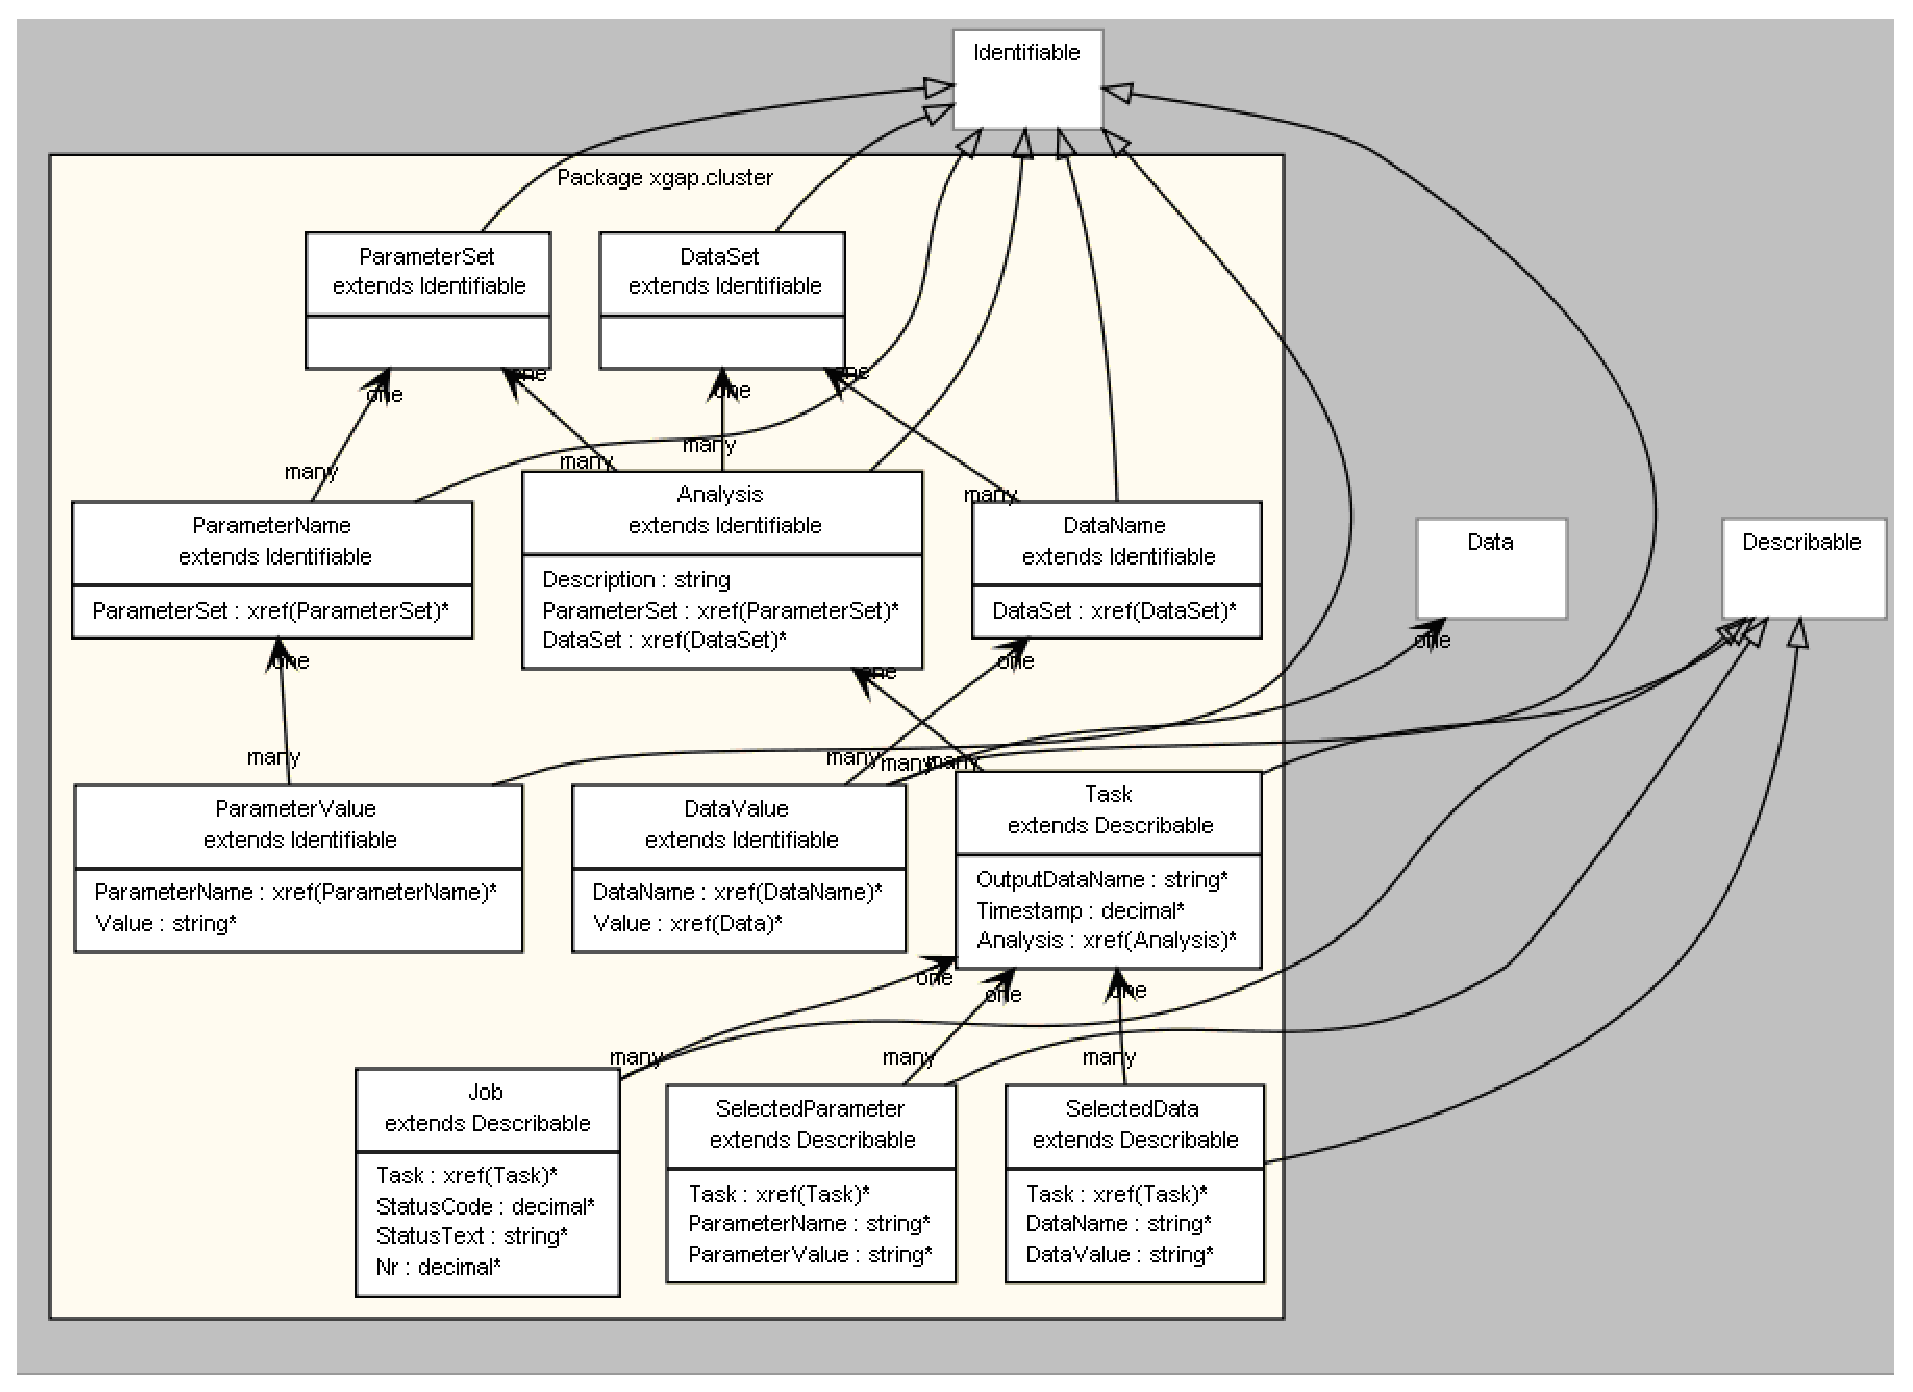
\includegraphics[height=8.0cm,width=15.0cm]{images/datamodel.eps}}
  \caption{Datamodel}
  \label{fig:FigDATAMODEL}    
\end{figure}

\begin{figure}[ht]  
\centering
  \hfill
  \fbox{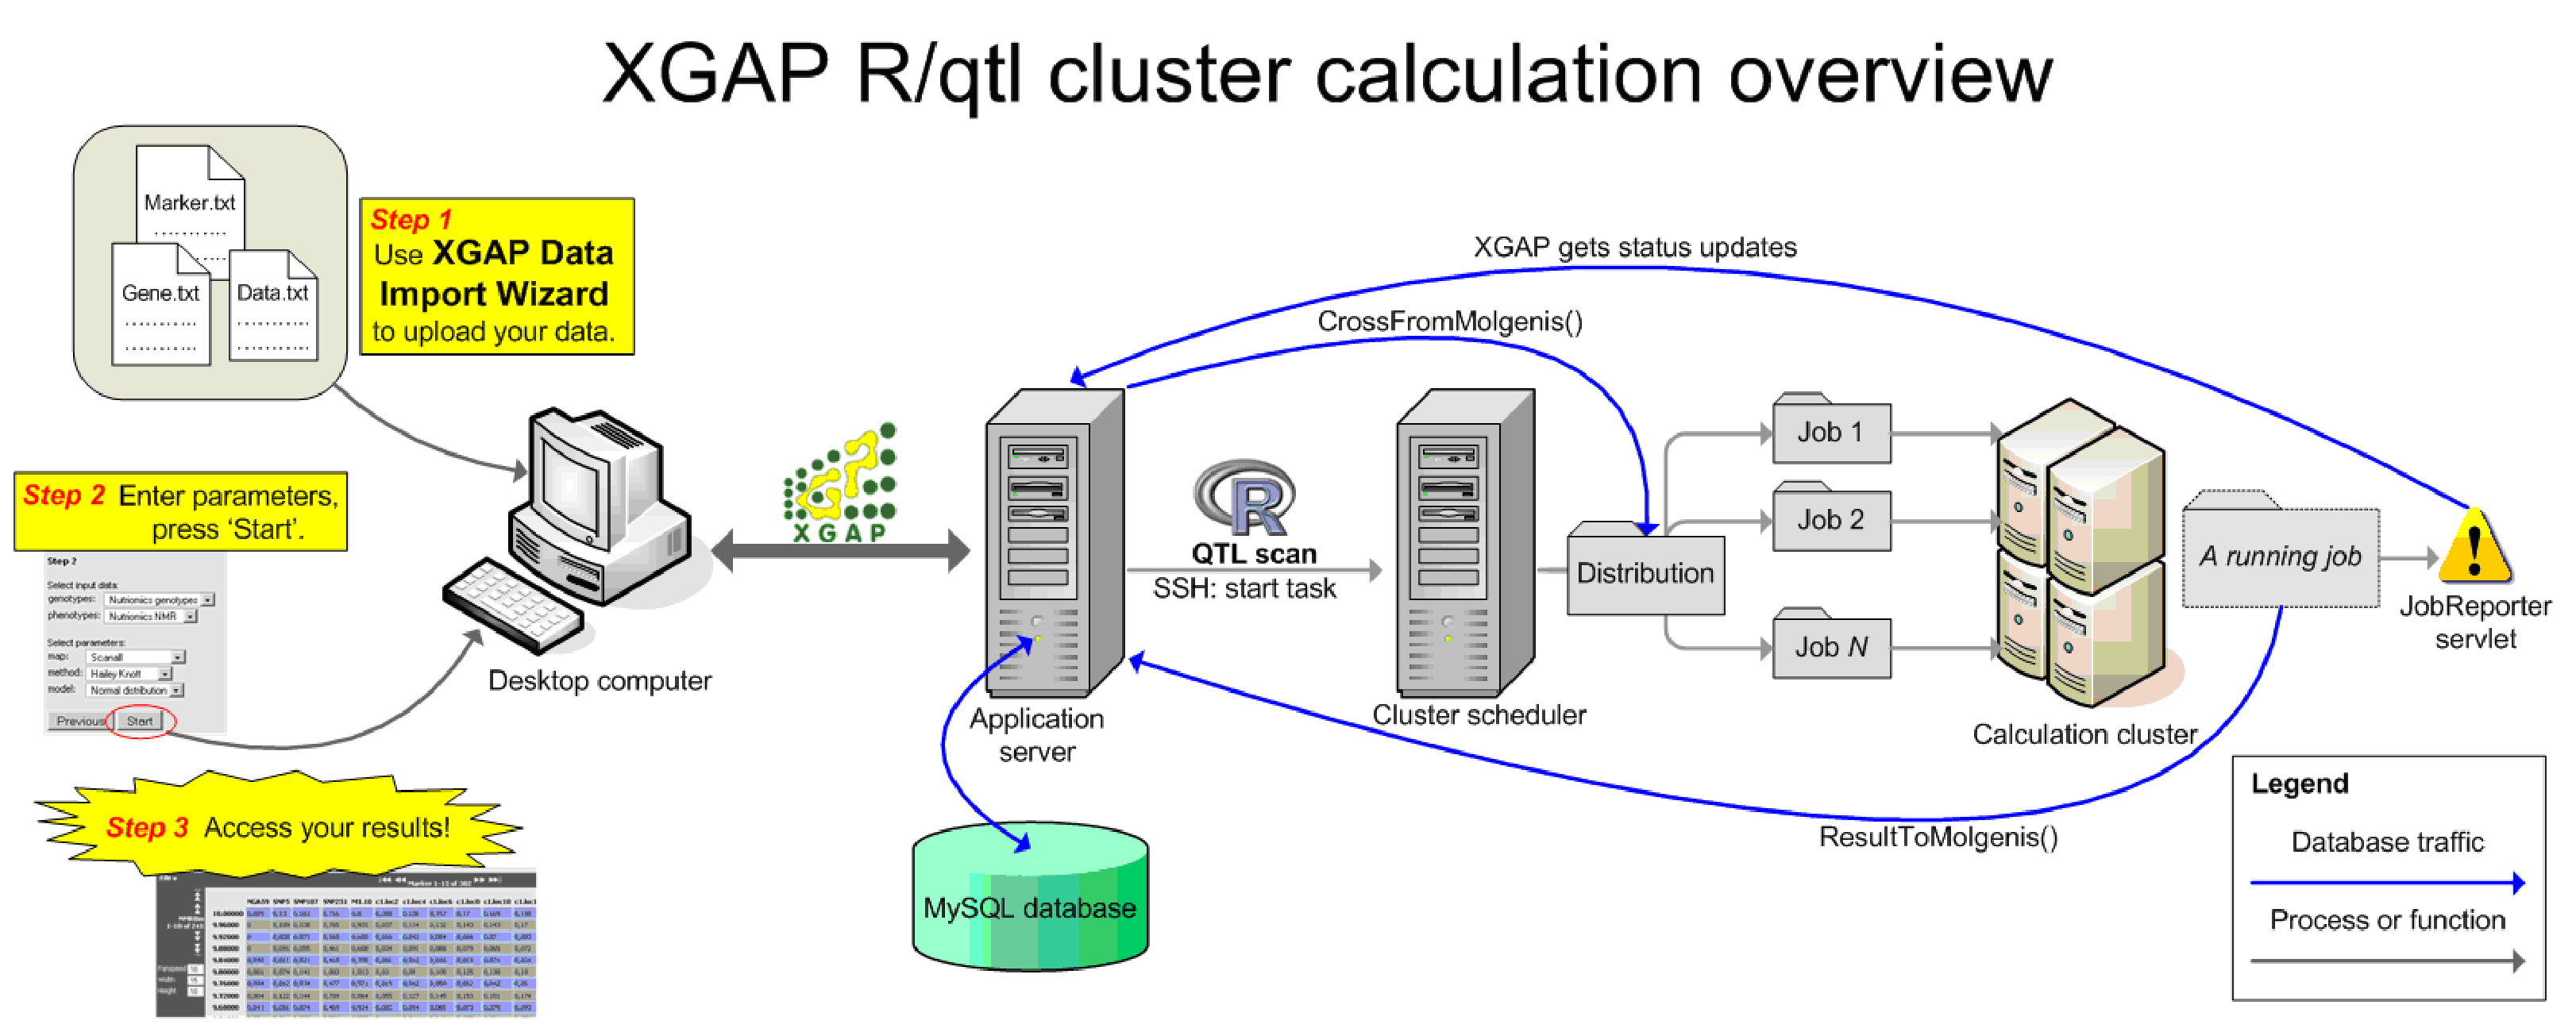
\includegraphics[height=8.0cm,width=15.0cm]{images/layout.eps}}
  \caption{Layout}
  \label{fig:FigLAYOUT}    
\end{figure}

\subsection{HPC of QTLs using molgenis}
Because there is a high threshold for biological users to use R for QTL analysis a webplugin into the molgenis system was created to enable users to 
use the molgenis webinterface to do highspeed parallelized QTL analysis. The plugin stores QTL profiles back into the database and also information about each run.
A webinterface provides users with a one click sollution, while the more complicated task are hidden out of sight. 
An overview of what happens out of sight can be seen in FIG XX.
The following functions are used during cluster analysis
\begin{itemize}
	\item CrossFromMolgenis() - Retrieving a dataset in the R/qtl cross format from a molgenis database system with the XGAP dataformat
	\item ResultsToMolgenis() - Storing results to a molgenis database system with the XGAP dataformat
	\item ResultsFromMolgenis() - Retrieving previously stored QTL analysis results from a molgenis database system with the XGAP dataformat
\end{itemize}

\begin{table}[ht]
	\caption{R/QTL parameters}
	\centering
	\begin{tabular}{| l | c | }
	\hline
	Scanall	&Main scanning interface of R/QTL created by K. Brohman et al\\
			&implementing per marker QTL analysis using different models and mapping methods.\\
	\hline
	MQMall	&Multiple QTL Mapping algorithm created by R.C. Janssen\\
			&implementing multiple QTL modeling and mapping using normal distributions.\\
	\hline
	CIMall	&Composite interval mapping created by G. Churchill and Senuk Sen\\
	\hline
	\end{tabular}
	\label{tbl:tabel0}
\end{table}

\begin{table}[ht]
	\caption{Reporter statuscodes}
	\centering
	\begin{tabular}{| l | c | c | }
	\hline
	-1	&Red	&An error has occurred.\\
	\hline
	0	&Orange	&Submitted to cluster as a potential job.\\
	\hline
	1	&Yellow	&Job is accepted and queued.\\
	\hline
	2	&Blue	&Job calculation done and is now uploading results back to the database.\\
	\hline
	3	&Green	&Job is completed.\\
	\hline
	\end{tabular}
	\label{tbl:tabel1}
\end{table}


\newpage
\section{Conclusions}
\subsection{Additions to R/qtl}
MQM was succesfully integrated into the R/qtl package, also several extension to R/qtl
were made which are summarized below. Also a manual to the R/qtl + mqm package was created together with Pjotr Prins, Richard Finkers, Ronnie Joosen and Karl Broman. The first drafts of a paper on the inclusion of MQM into R/qtl can be found in the additional materials section.
\begin{itemize}
\item Parallel multitrait analysis implemented into R/qtl using the SNOW library to utilize multi cpu desktop machines
\item Parallel single trait permutation analysis implemented into R/qtl
\item Parallel genomewide permutation and FDR implemented into R/qtl
\item Plotting routines to visualize multitrait and bootstrap analysis to graphically investigate large amounts of QTL profiles
\item Added the option to retrieve structured datasets from a XGAP/MolgenisDB
\item Added the option to store and retrieve results from a XGAP/MolgenisDB
\item Added a additional scanning function mqm implementing the multiple QTL mapping (MQM) algorithm
\item For all functions added to the R/qtl package helpfiles were created with executable examples for each function.
\end{itemize}
\subsection{HPC QTL using the Molgenisplugin}
A plugin for the Molgenis database system using XGAP was created, to enable Molgenis users to do R/qtl analysis using a HPC cluster.
Also QTL analysis can be performed on the localserver of the Molgenis database. Thus removing the need for a HPC cluster, and adding more flexibility to the plugin system. Using localserver QTL analysis a user doesn't benefit from the decrease in calculation time, because jobs are calculated sequentially. An online example of parallel QTL mapping using the RUG HPC cluster can be found at:\\
http:$\backslash$$\backslash$gbic.target.rug.nl:8080$\backslash$xgap4clusterdemo$\backslash$ \\

\section{Discussion}
\subsection{Datastructuring and storage via: XGAPDB}

\subsection{HPC of QTLs using molgenis}
Further extensions of the plugin currently under development:
\begin{itemize}
	\item - A priori checking of tables selected
	\item - Expose more scanning routines (CIM,MQM)
	\item - Expose all available parameters (scanone,CIM,MQM)
	\item - Better required time estimation of runtime on cluster
	\item - Concurrent runs
	\item - Better status overview using active polling of the calculationserver
\end{itemize}
\newpage
\section{Literature}
 \begin{thebibliography}{9}
	\bibitem{budding02}
		Rachel B. Brem, et al.; 2002.
		\emph{Genetic Dissection of Transcriptional Regulation in Budding Yeast}
		Science 296, 752.
	\bibitem{eQTL1}
		Breitling R, Li Y, Tesson BM, Fu J, Wu C, et al.; 2008 
		\emph{Genetical Genomics: Spotlight on QTL Hotspots.}
		PLoS Genetics 4 (10).
	\bibitem{eQTL2}
		Bystrykh L, Weersing E, Dontje B, Sutton S, Pletcher MT, Wiltshire T, Su AI, Vellenga E, Wang J, Manly KF, Lu L, Chesler EJ, Alberts R, Jansen RC, Williams RW, Cooke MP, de Haan G.; 2005
		\emph{Uncovering regulatory pathways that affect hematopoietic stem cell function using genetical genomics.}
		Nature Genetics  37, 225 - 232 
	\bibitem{eQTL3}
		Li, Y.; Alda Alvarez, O.; Gutteling, E.W.; Tijsterman, M.; Fu, J.; Riksen, J.A.G.; Hazendonk, E.; Prins, J.C.P.; Plasterk, R.H.A.; Jansen, R.C.; Breitling, R.; Kammenga, J.E.; 2006
		\emph{Mapping Determinants of Gene Expression Plasticity by Genetical Genomics in C. elegans}
		Plos Genetics 2 (12). - p. 0001 - 0007. 		
	\bibitem{broman09}
		Broman, K.W.; 2009.
		\emph{A brief tour of R/qtl}
		http:$\backslash$$\backslash$www.rQTL.org, R/qtl tutorials.
	\bibitem{broman03}
		Broman, K.W.; Wu, H.; Sen, S.; Churchill, G.A.; 2003.
		\emph{R/qtl: QTL mapping in experimental crosses}
		Bioinformatics, 19:889-890.
	\bibitem{keurtj}
		Keurentijes JJB, Fu J, de Vos CHR,Lommen A, Jansen RC et al; 2006.
		\emph{The genetics of plant metabolism.}
		Nature Genetics. 38, 842�849. 
	\bibitem{Oats}
		L.S. O'Donoughue, S.F. Kianian, P.J. Rayapati, G.A. Penner, M.E. Sorrells,
		S.D. Tanksley, R.L. Phillips, H.W. Rines, M. Lee, G. Fedak, S.J. Molnar, 
		D. Hoffman, C.A. Salas, B. Wu, E. Autrique and A. Van Deynze;  1995.  
		\emph{A molecular linkage map of cultivated oat.}
		Genome 38:368-380
	\bibitem{Hyper}
		Sugiyama, F., Churchill, G. A., Higgens, D. C., Johns, C., Makaritsis, K. P., Gavras, H. Paigen, B; 2001.
		\emph{Concordance of murine quantitative trait loci for salt-induced hypertension with rat and human loci.}
		Genomics 71, 70�77. 
	\bibitem{Listeria}
		Boyartchuk, V. L., Broman, K. W., Mosher, R. E., D'Orazio S. E. F., Starnbach, M. N. Dietrich, W. F; 2001.
		\emph{Multigenic control of Listeria monocytogenes susceptibility in mice.}
		Nature Genetics 27, 259�260. 
	\bibitem{jansen07}
		Jansen R. C.; 2007.
		\emph{Chapter 18 - Quantitative trait loci in inbred lines} 
		Handbook of Stat. Genetics 3th edition,(c) 2007 John Wiley \& Sons, Ltd.
	\bibitem{tierney04}	
		Tierney, L.; Rossini, A.; Li, N.; Sevcikova, H.; 2004.
		\emph{The snow Package: Simple Network of Workstations} Version 0.2-1. 
	\bibitem{tierney03}
		Rossini, A.; Tierney, L.; Li, N.; 2003.
		\emph{Simple parallel statistical computing}
		R. UW Biostatistics working paper series University of Washington. 193
	\bibitem{jansen01}	
		Jansen R. C.; Nap J.P.; 2001
		\emph{Genetical genomics: the added value from segregation}
		Trends in Genetics, 17, 388-391.
	\bibitem{jansen94}		
		Jansen R. C.; Stam P.; 1994
		\emph{High resolution of quantitative traits into multiple loci via interval mapping}
		Genetics, 136, 1447-1455. 
	\bibitem{Churchill94}
		Churchill, G. A.; Doerge, R. W.; 1994
		\emph{Empirical threshold values for quantitative trait mapping}
		Genetics 138, 963�971. 
	\bibitem{jansen93}
		Jansen R. C.; 1993
		\emph{Interval mapping of multiple quantitative trait loci}
		Genetics, 135, 205�211.
	\bibitem{PBS2000}
		Veridian Information Solutions; 2000
		\emph{Portable Batch System - OpenPBS Release 2.3:Administrator Guide}
		website at: www.veridian.com.
	\bibitem{Dempster77}
		Dempster, A. P.; Laird, N. M. and Rubin, D. B.; 1977 
		\emph{Maximum likelihood from incomplete data via the EM algorithm}
		J. Roy. Statist. Soc. B, 39, 1�38.
	\bibitem{Rcurl08}
		Temple Lang D. ; 2008
		\emph{R as a Web Client � the RCurl package}
		Journal of Statistical Software
	\bibitem{brouwer09}
		Brouwer R. 2008/2009;
		\emph{Code from various research projects}
		GBB: MolGen Groningen
	\bibitem{morris07}
		Swertz MA, Jansen R. C.; 2007
		\emph{Beyond standardization: dynamic software infrastructures for systems biology}
		Nat Rev Genet. 3, 235�243. 
	\bibitem{morris04}
		Swertz M.A., De Brock E.O., Van Hijum S.A., De Jong A., Buist G., Baerends R.J., Kok J., Kuipers O.P., Jansen R.C.; 2004.
		\emph{Molecular Genetics Information System (MOLGENIS): Alternatives in developing local experimental genomics databases}
		Bioinformatics,13, 2075�2083.
	\bibitem{mapQTL}
		Van Ooijen \& Maliepaard; 1996
		\emph{MapQTL version 3.0: Software for the calculation of QTL positions on genetic maps.}
		Plant Genome IV Abstracts, http://www.intl-pag.org.
	\bibitem{Rpara}
		Gonzalo V., Jansen R.C.  and Suppi R.L. ; 2008
		\emph{R/parallel � speeding up bioinformatics analysis with R}
		BMC Bioinformatics 2008, 9:390
\end{thebibliography}
\newpage
\section{Additional information}
\subsection*{Script \& Code}
Script and code created and used can be found at:\\
http:$\backslash$$\backslash$github.com$\backslash$DannyArends\\
http:$\backslash$$\backslash$github.com$\backslash$DannyArends$\backslash$rqtl-mqm\\
http:$\backslash$$\backslash$github.com$\backslash$DannyArends$\backslash$MolgenisInterface\\

\subsection*{Additional tables}
Tables \ref{tbl:tabel1} \& \ref{tbl:tabelCluster} list the dependencies needed to use the software discribed in this thesis. 
The scriptfile QTLanalysis.R ,dependency for functioning of the clusterservice,
can be found inside the molgenispackage.
Tables \ref{tbl:tabel3} \& \ref{tbl:tabel2} made using R/qtl "Map10" dataset, for scanone bootstrapping parameters were: 
500 bootstraps in batches of 50 at a time on a simulated F2 population with \# individuals as stated in column 1 (Table \ref{tbl:tabel2}).
For mqm we used 50 bootstraps in batches of 5 (Table \ref{tbl:tabel3}). Runs were performed using standard setting for each algorithm. 
Profiling code is available at request.\\

\begin{table}[ht]
	\caption{Requirements for using the R/qtl package}
	\centering
	\begin{tabular}{| l | c | }
	\hline
	Operating system(s):&platform independent\\
	Programming languages:&R, C++\\
	Programs:&R 2.8.0\\
	Dependencies:&SNOW\cite{tierney04}\\
	Published using:&GNU 2 licence\\
	\hline
	\end{tabular}
	\label{tbl:tabel1}
\end{table}

\begin{table}[ht]
	\caption{Requirements for using R/qtl on a cluster}
	\centering
	\begin{tabular}{| l | c | }
	\hline
	Operating system(Cluster):&Unix / Linux\\
	Operating system(Webservice):&platform independent\\
	Programs(Cluster):&R 2.8.0\\
	&PBS\\
	Programs(Webservice):&Molgenis 3.3 Distro\\
	&XGAP 1.1\\
	Dependencies(Cluster):&molgenispackage\\
	&R/qtl\\
	&RCurl\cite{Rcurl08}\\
	&QTLanalysis.R\\
	Dependencies(Webservice):&webserver(APACHE)\\
	&database(mySQL)\\
	&Eclipse Ganymede (Developers)\\
	Published using:&GNU 2 licence\\
	\hline
	\end{tabular}
	\label{tbl:tabelCluster}
\end{table}

\begin{table}[ht]
	\caption{Profiling bootstrap analysis of scanone using a QuadCore machine}
	\centering
	\begin{tabular}{| l | l | l | l | l | c | c | c |}
	\hline
	\# Individuals & Single & Ncore=2 & Ncore=3 & Ncore=4 & \%2vs1 & \%3vs1 & \%4vs1\\
	\hline
	\hline
	10 & 83.00 & 68.00 & 65.00 & 65.00 & -18.1\% & -21.7\% & -21.7\%\\
	20 & 91.00 & 72.00 & 67.00 & 67.00 & -20.9\% & -26.4\% & -26.4\%\\
	50 & 118.00 & 84.00 & 76.00 & 74.00 & -28.8\% & -35.6\% & -37.3\%\\
	100	& 161.00 & 104.00 & 90.00 & 85.00 & -35.4\% & -44.1\% & -47.2\%\\
	200	& 251.00 & 146.00 & 118.00 & 107.00 & -41.8\% & -53.0\% & -57.4\%\\
	350	& 377.00 & 204.00 & 158.00 & 138.00 & -45.9\% & -58.1\% & -63.4\%\\
	500	& 501.00 & 261.00 & 198.00 & 169.00 & -47.9\% & -60.5\% & -66.3\%\\
	750	& 709.00 & 359.00 & 263.00 & 220.00 & -49.4\% & -62.9\% & -69.0\%\\
	1000 & 919.00 & 453.00 & 329.00 & 271.00 & -50.7\% & -64.2\% & -70.5\%\\
	2000 & 1754.00 & 840.00 & 593.00 & 477.00 & -52.1\% & -66.2\% & -72.8\%\\
	\hline
	\end{tabular}
	\label{tbl:tabel3}
\end{table}

\begin{table}[ht]
	\caption{Profiling analysis using a DualCore machine}
	\centering
	\begin{tabular}{| l | l | l | l | c |}
	\hline
	\# Individuals &	Method &	Single (sec) &	N.core=2 (sec) & \% Improvement (\%) \\
	\hline
	\hline
	10	& scanone &	103.00 &	85.00 &	17.5\%\\
	20	& scanone &	115.00&	90.00&	21.7\%\\
	50	& scanone &	149.00&	107.00&	28.2\%\\
	100	& scanone &	205.00&	133.00&	35.1\%\\
	200	& scanone &	318.00&	187.00&	41.2\%\\
	350	& scanone &	479.00&	266.00&	44.5\%\\
	500	& scanone &	645.00&	339.00&	47.4\%\\
	750	& scanone &	915.00&	465.00&	49.2\%\\
	1000 & scanone &	1186.00&	555.00&	53.2\%\\
	\hline
	10	&mqm&	143.00&	88.00&	38.5\%\\
	20	&mqm&	177.00&	99.00&	44.1\%\\
	50	&mqm&	211.00&	107.00&	49.3\%\\
	100	&mqm&	237.00&	133.00&	43.9\%\\
	200	&mqm&	347.00&	186.00&	46.4\%\\
	350 &mqm&	501.00&	270.00&	46.1\%\\
	500	&mqm&	646.00&	358.00&	44.6\%\\
	750	&mqm&	962.00&	505.00&	47.5\%\\
	1000 &mqm&	1311.00&	700.00&	46.6\%\\
	\hline
	\end{tabular}
	\label{tbl:tabel2}
\end{table}

\begin{table}[h!t]
	\caption{Profiling scalability of MQM}
	\centering
	\begin{tabular}{| l | l | l | l | l | l | l | l | l |}
	\hline
	\# Ind & \# Chr  & Length Chr & Markers & Stepsize & Stepped chr & Cof Each & Traits & Time (min)\\
	\hline
	\hline
	50 & 10 & 200 & 10*10 & 5 & 0-200 & 0 & 1 & 1.83\\
	100 & 10 & 200 & 10*10 & 5 & 0-200 & 0 & 1 & 2.17\\
	200 & 10 & 200 & 10*10 & 5 & 0-200 & 0 & 1 & 2.91\\
	400 & 10 & 200 & 10*10 & 5 & 0-200 & 0 & 1 & 4.14\\
	800 & 10 & 200 & 10*10 & 5 & 0-200 & 0 & 1 & 7.08\\	
	\hline
	100 & 1 & 200 & 100*1 & 5 & 0-200 & 0 & 1 & 0.48\\
	100 & 5 & 200 & 20*5 & 5 & 0-200 & 0 & 1 & 1.22\\
	100 & 10 & 200 & 10*10 & 5 & 0-200 & 0 & 1 & 2.91\\
	100 & 20 & 200 & 5*20 & 5 & 0-200 & 0 & 1 & 4.17\\
	\hline
	100 & 10 & 50 & 10*10 & 5 & 0-200 & 0 & 1 & 2.28\\
	100 & 10 & 100 & 10*10 & 5 & 0-200 & 0 & 1 & 2.19\\
	100 & 10 & 200 & 10*10 & 5 & 0-200 & 0 & 1 & 2.19\\
	\hline
	100 & 10 & 200 & 10*10 & 1 & 0-200 & 0 & 1 & 9.13\\
	100 & 10 & 200 & 10*10 & 2 & 0-200 & 0 & 1 & 4.81\\
	100 & 10 & 200 & 10*10 & 5 & 0-200 & 0 & 1 & 2.19\\
	100 & 10 & 200 & 10*10 & 10 & 0-200 & 0 & 1 & 1.28\\
	100 & 10 & 200 & 10*10 & 20 & 0-200 & 0 & 1 & 0.82\\
	\hline
	100 & 10 & 200 & 10*10 & 5 & 0-200 & 8 & 1 & 1.7\\
	100 & 10 & 200 & 10*10 & 5 & 0-200 & 5 & 1 & 2.13\\
	100 & 10 & 200 & 10*10 & 5 & 0-200 & 3 & 1 & 3.14\\
	100 & 10 & 200 & 10*10 & 5 & 0-200 & 2 & 1 & 5.94\\
	\hline
	800 & 10 & 200 & 50*10 & 5 & 0-200 & 8 & 1 & 79.29\\
	400 & 10 & 200 & 50*10 & 5 & 0-200 & 8 & 1 & 42.51\\
	100 & 10 & 200 & 50*10 & 5 & 0-200 & 8 & 1 & 14.22\\
	\hline
	\end{tabular}
	\label{tbl:tabel4}
\end{table}

\begin{table}[h!t]
	\caption{R/qtl parameters}
	\centering
	\begin{tabular}{| l | l | }
	\hline
	&\bf QTL mapping method\\
	\hline
	Scanall	&Main scanning interface of R/qtl created by K. Broman et al\\
			&implementing per marker QTL analysis using different models \\
			&and mapping methods.\\
	\hline
	MQMall	&Multiple QTL Mapping algorithm created by R.C. Janssen\\
			&implementing multiple QTL modeling and mapping using normal\\ 
			&distributions.\\
	\hline
	CIMall	&Composite interval mapping created by G. Churchill and \\
			&Senuk Sen\\
	\hline
	&\bf QTL trait model\\
	\hline
	Normal & Used for traits that follow a normal distribution\\
	\hline
	2part & 2-part model\\
	\hline
	Binary & Used for binary traits\\
	\hline
	Non-Parametric & Used when none of the other models fit the trait\\
		&data (least power)\\
	\hline
	&\bf Method of mapping QTLs\\
	\hline
	em & EM Algorithm\\
	\hline
	imp & Imputation\\
	\hline
	hk & Hailey-Knott regression\\
	\hline
	ehk & extended Hailey-Knott\\
	\hline
	mr & Basic marker regression (removing unknowns)\\
	\hline
    mr-imp & marker regression by single imputation of unknown values\\
	\hline
	mr-argmax & Marker regression using the viterbi algorithm to estimate \\
	& unknown values\\
	\hline
	\end{tabular}
	\label{tbl:tabelPARAMS}
\end{table}

\begin{table}[h!t]
	\caption{Taskreporter plugin status codes}
	\centering
	\begin{tabular}{| l | c | c | }
	\hline
	-1	&Red	&An error has occurred.\\
	\hline
	0	&Orange	&Submitted to cluster as a potential job.\\
	\hline
	1	&Yellow	&Job is accepted and queued.\\
	\hline
	2	&Blue	&Job is running.\\
	\hline
	3	&Green	&Job is completed.\\
	\hline
	\end{tabular}
	\label{tbl:tabelSTATUS}
\end{table}
\clearpage
\subsection*{Additional figures}
	\begin{figure}[ht]
	  \hfill
	  \fbox{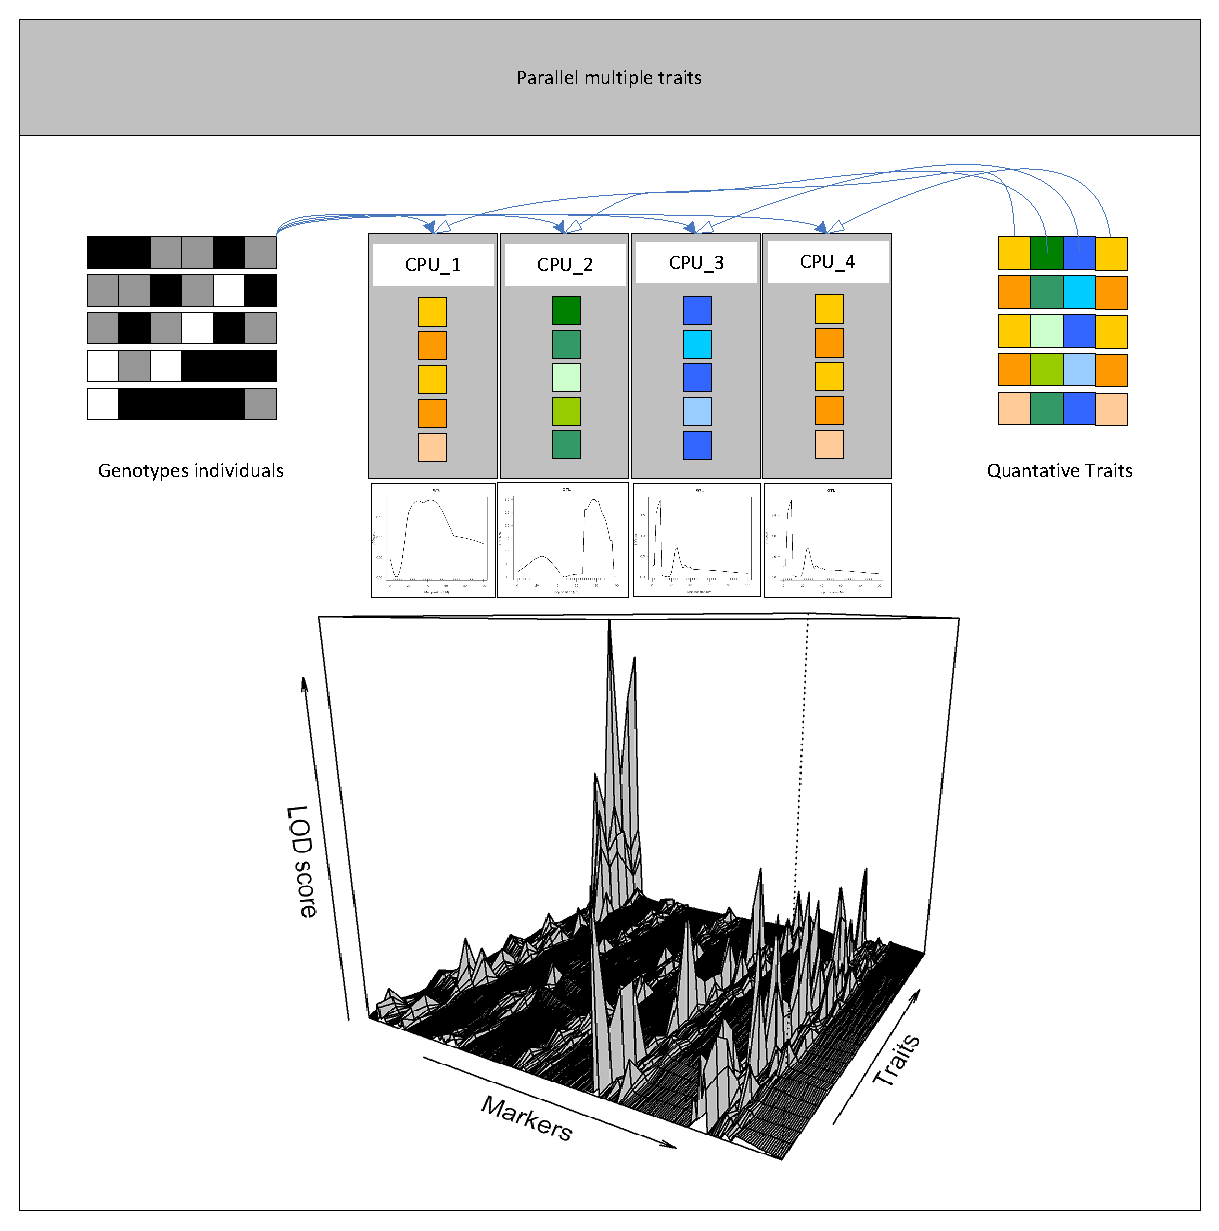
\includegraphics[height=5.0cm,width=10.0cm]{Images/MT_small_newer.eps}}
	  \caption{Overview of the way many endophenotypes are analysed using multiple cores. Tasks are split linearly and distributed across available cores ($Here: \# core = \# traits$, with $traits > cores$ traits are batched into jobs, which are then distributed across cores.)}
	  \label{fig:MTstrait}
	\end{figure}
	
	\begin{figure}[ht]
	  \hfill
	  \fbox{\includegraphics[height=8.0cm,width=12.0cm]{Images/MTperm.eps}}
	  \caption{Overview of the way many endophenotypes permutation using multiple cores. Tasks consist of a single permutation of the data keeping trait correlation intact. Tasks are split linearly and distributed across available cores ($Here: \# core = \# traits$, with $traits > cores$ traits are batched into jobs, which are then distributed across cores.)}
	  \label{fig:MTperm}
	\end{figure}
	
	\begin{figure}[ht]
	  \hfill
	  \fbox{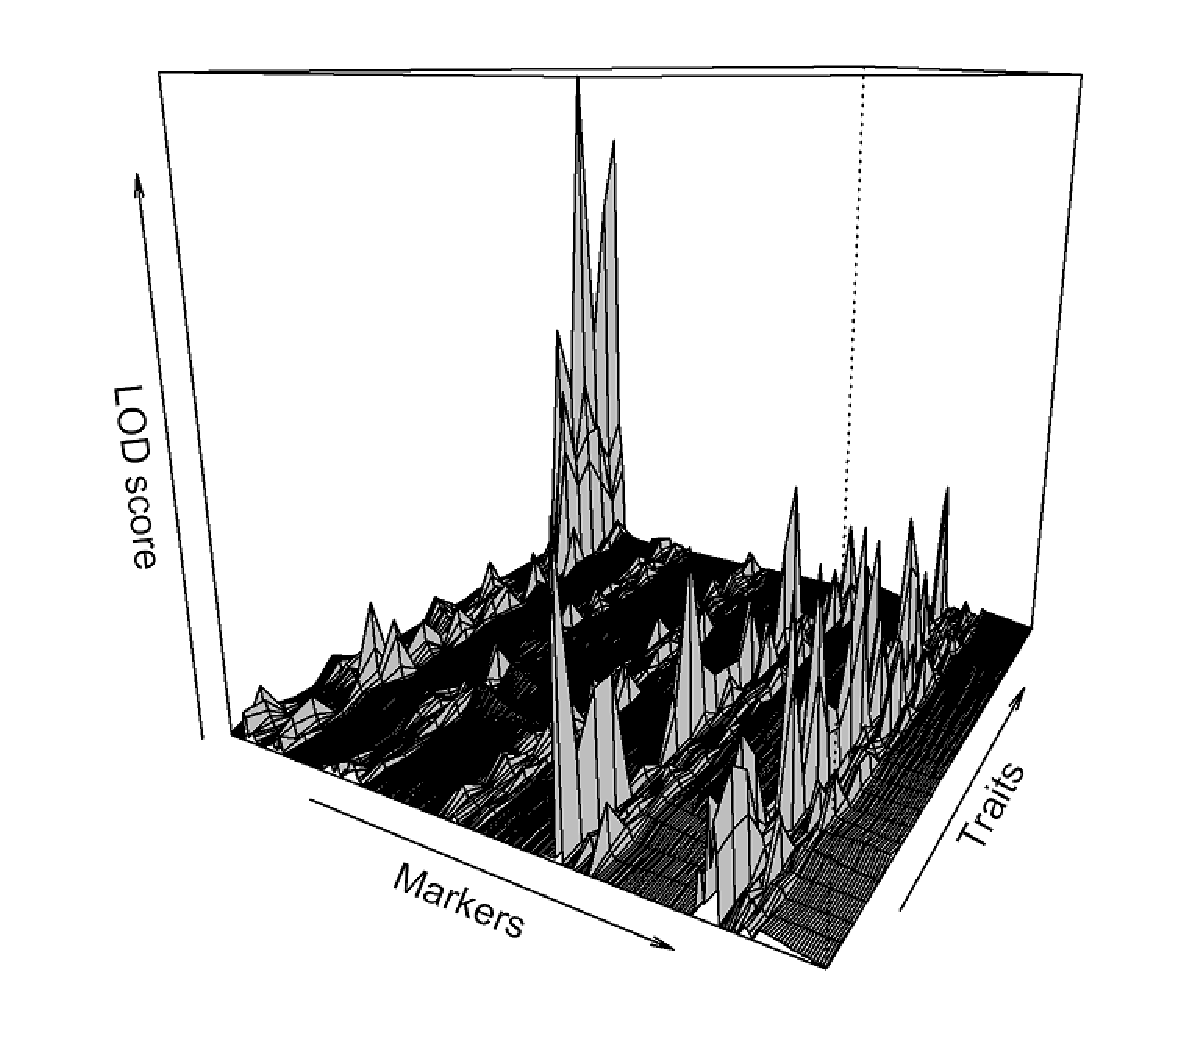
\includegraphics[height=8.0cm,width=12.0cm]{Images/multi3d.eps}}
	  \caption{Example of new ploting routine: Many endophenotypes analyses on 24 traits of the example dataset: "multitrait", displayed in 3D mode}
	  \label{fig:FigureThreeD}
	\end{figure}
	
	\begin{figure}[ht]  
	  \hfill
	  \fbox{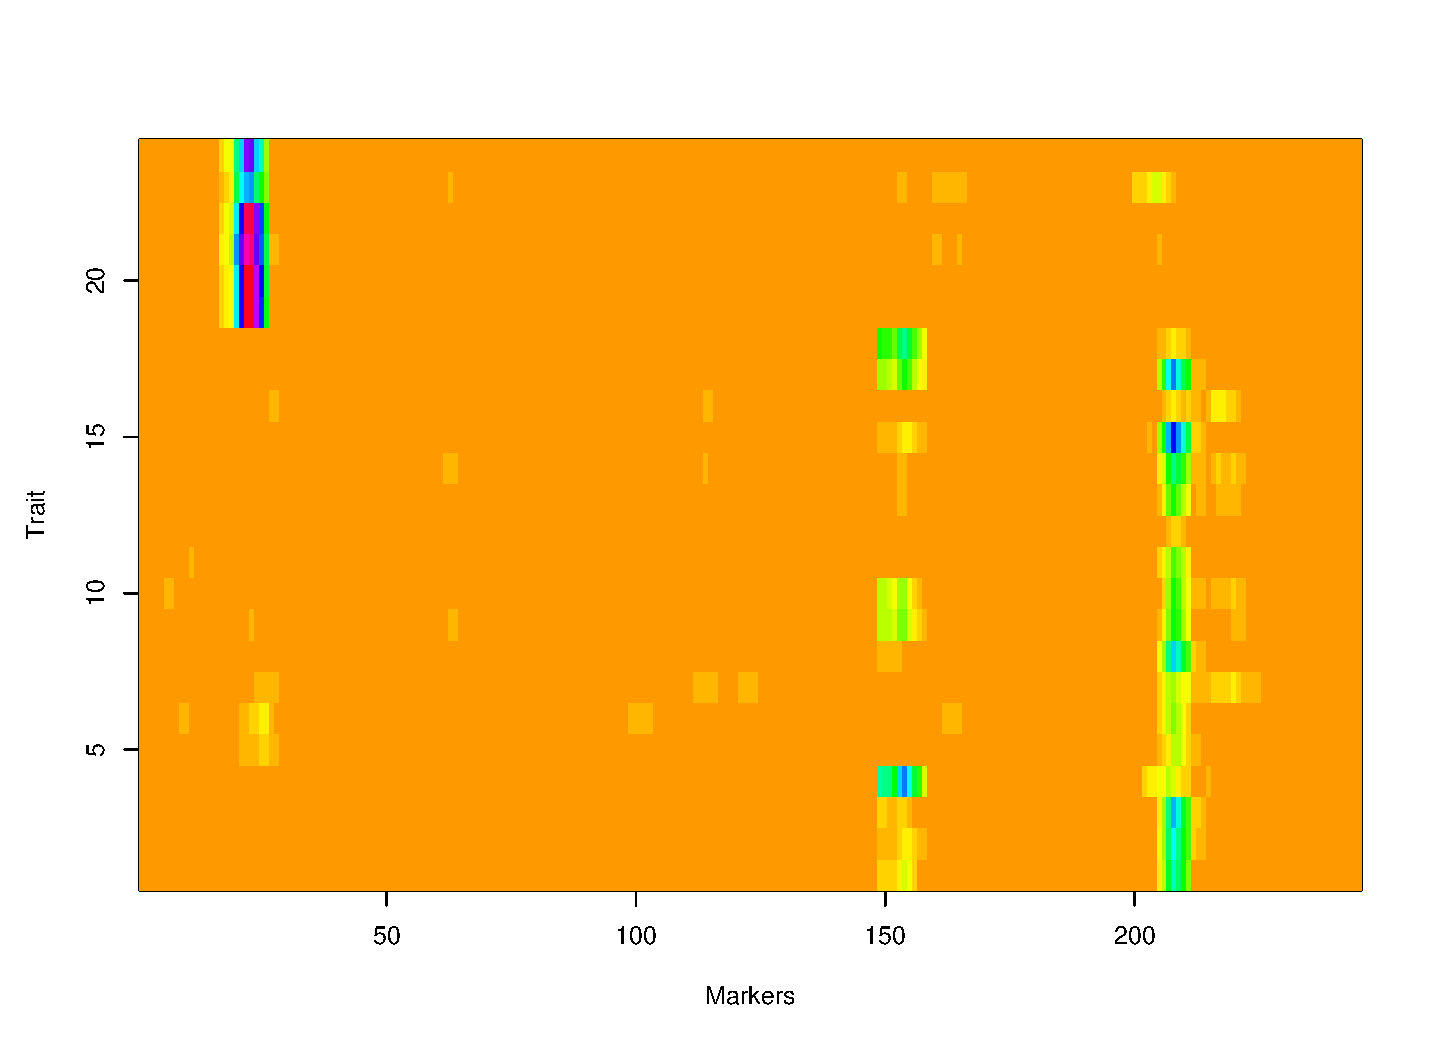
\includegraphics[height=8.0cm,width=12.0cm]{Images/multiHeat.eps}}
	  \caption{Example of new ploting routine: Many endophenotypes analyses analysis on the 24 traits of the example dataset: "multitrait", as a heatmap}
	  \label{fig:FigureHeat}    
	\end{figure}
	
	\begin{figure}[ht]  
	  \hfill
	  \fbox{\includegraphics[height=8.0cm,width=12.0cm]{Images/bootstrap12500.eps}}
	  \caption{Example of new ploting routine: Bootstrap analysis on trait 6 of the example dataset: "multitrait". In this picture the dashed green line represents a 5\% significance threshold, the blue a 10\%.}
	  \label{fig:FigureBoot}
	\end{figure}
	
	\begin{figure}[ht]
	  \hfill
	  \fbox{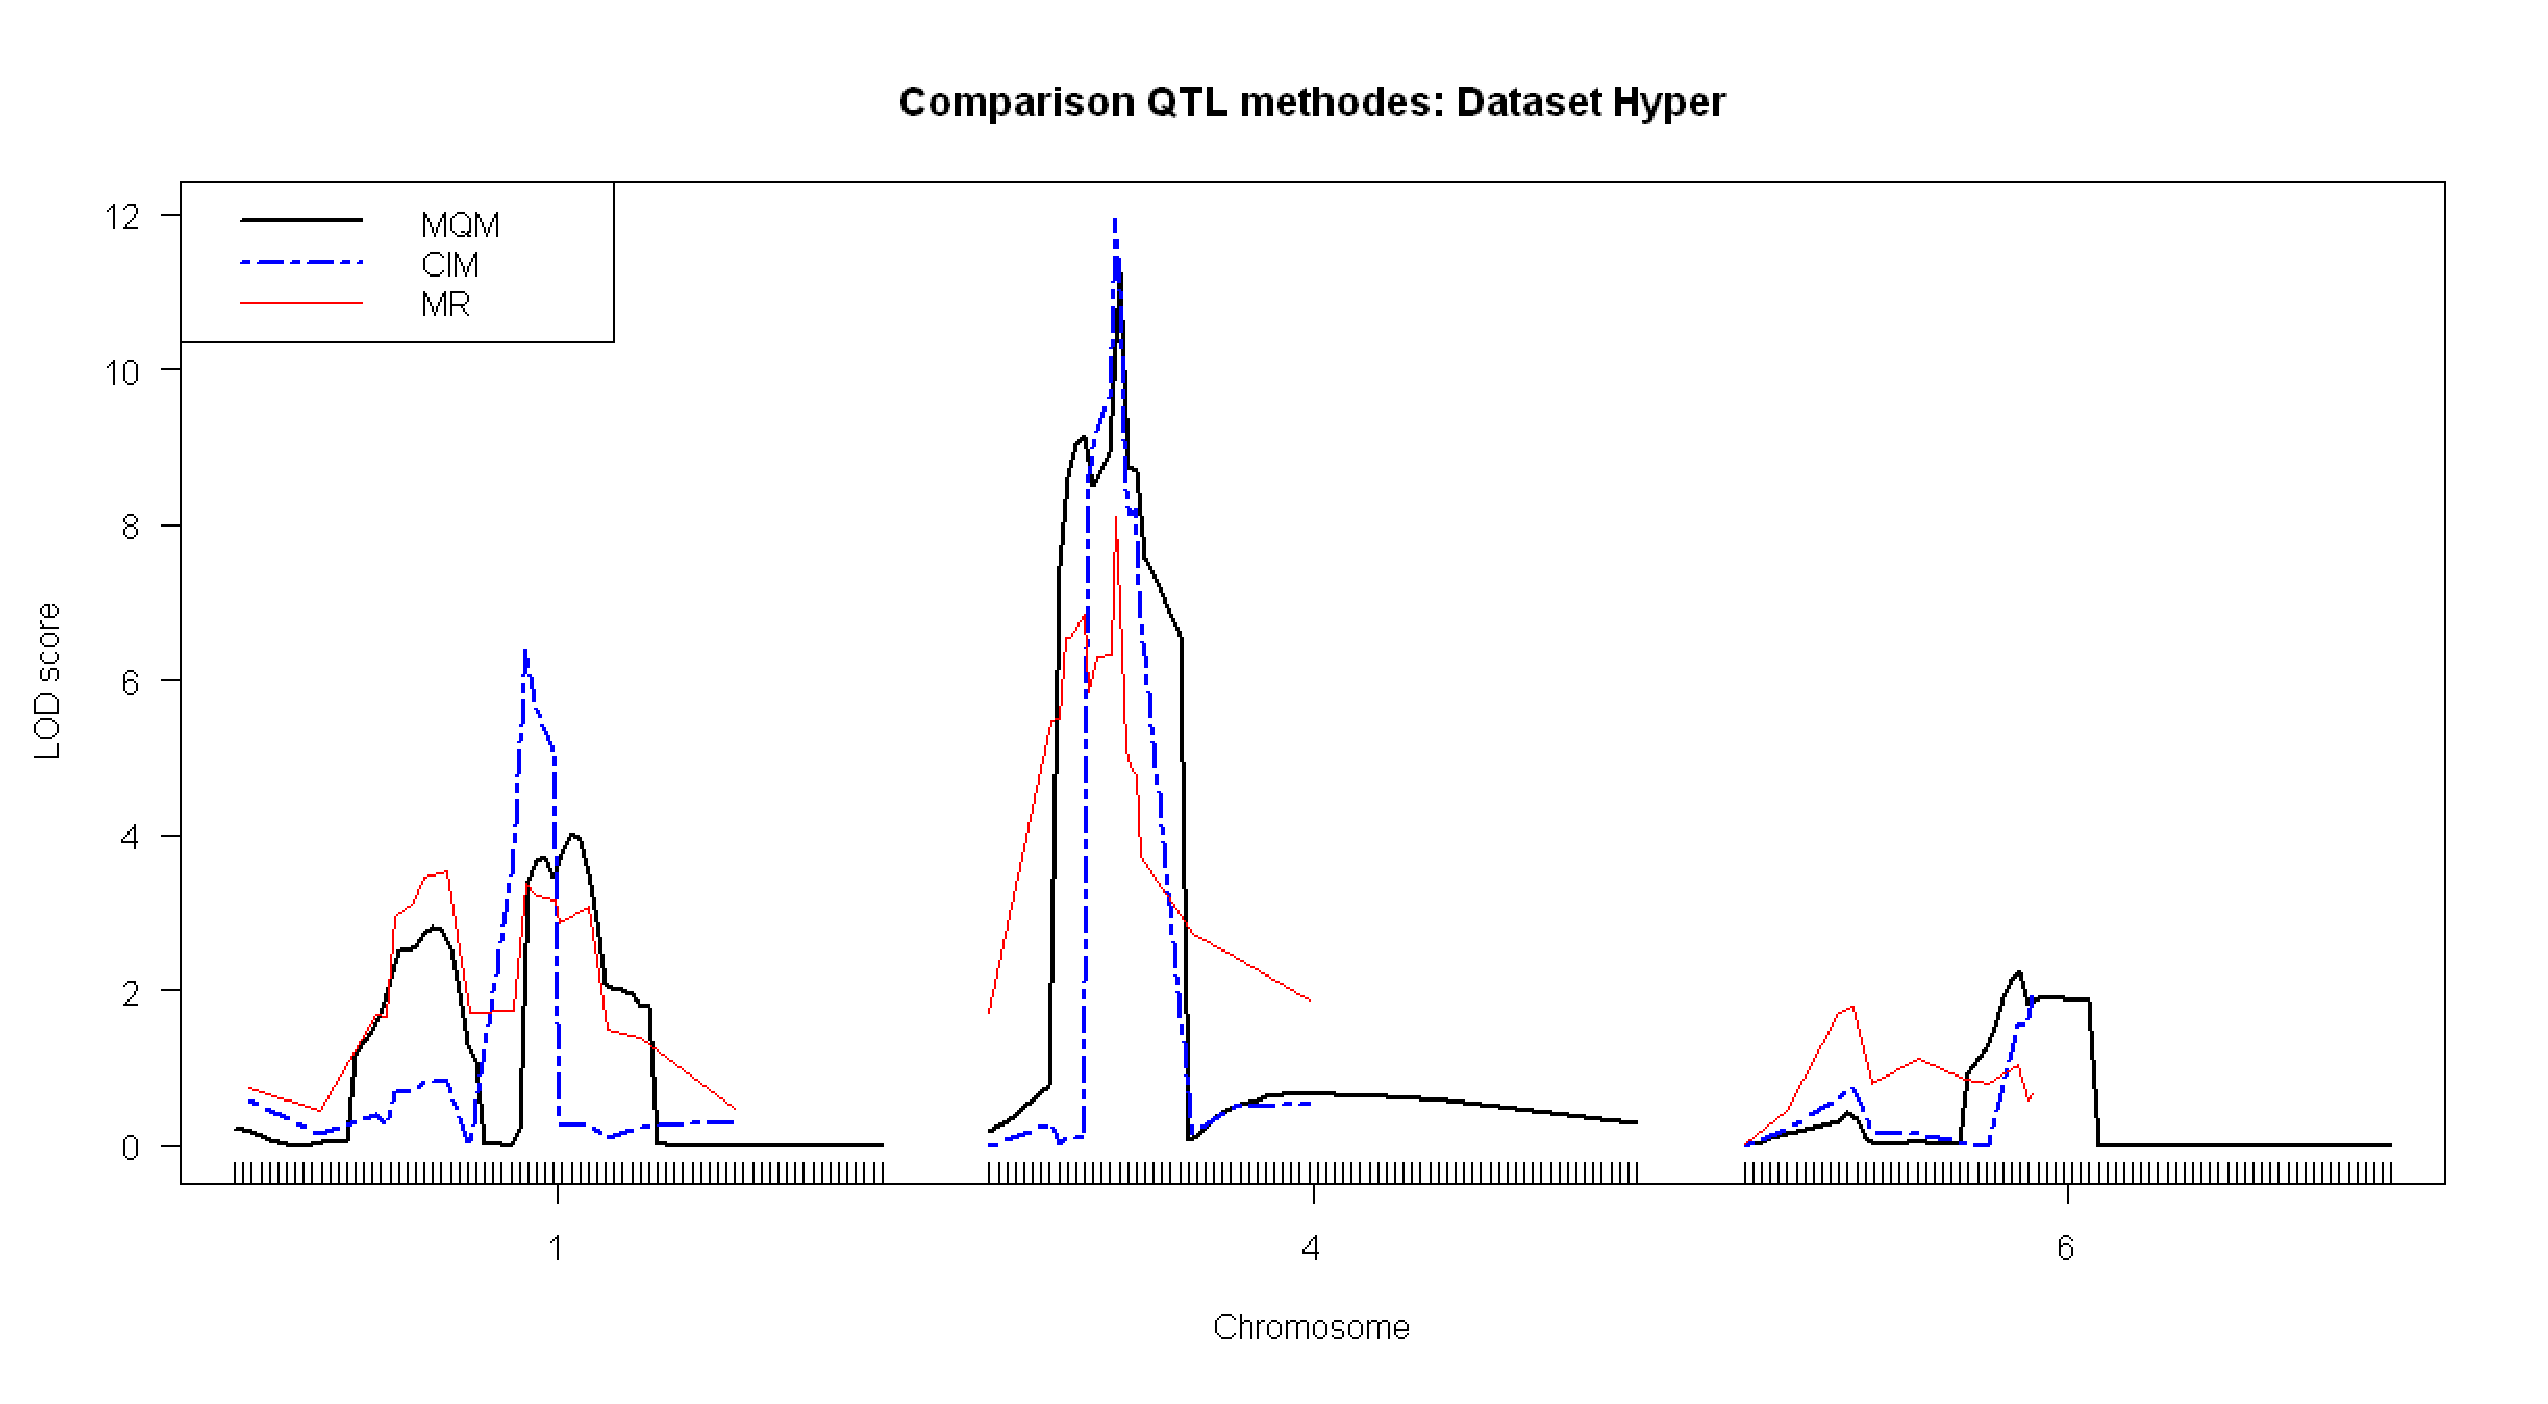
\includegraphics[height=8.0cm,width=12.0cm]{Images/DatasetHyper.eps}}
	  \caption{MQM in comparison with other QTLmapping methods (CIM, MR) using the dataset: "hyper". Using MQM we set cofactors every third marker, and do backward selection using a windowsize of 15 Cm. CIM also uses a window of 15Cm}
	  \label{fig:FigureHyper}
	\end{figure}
	
	\begin{figure}[ht]
	  \hfill
	  \fbox{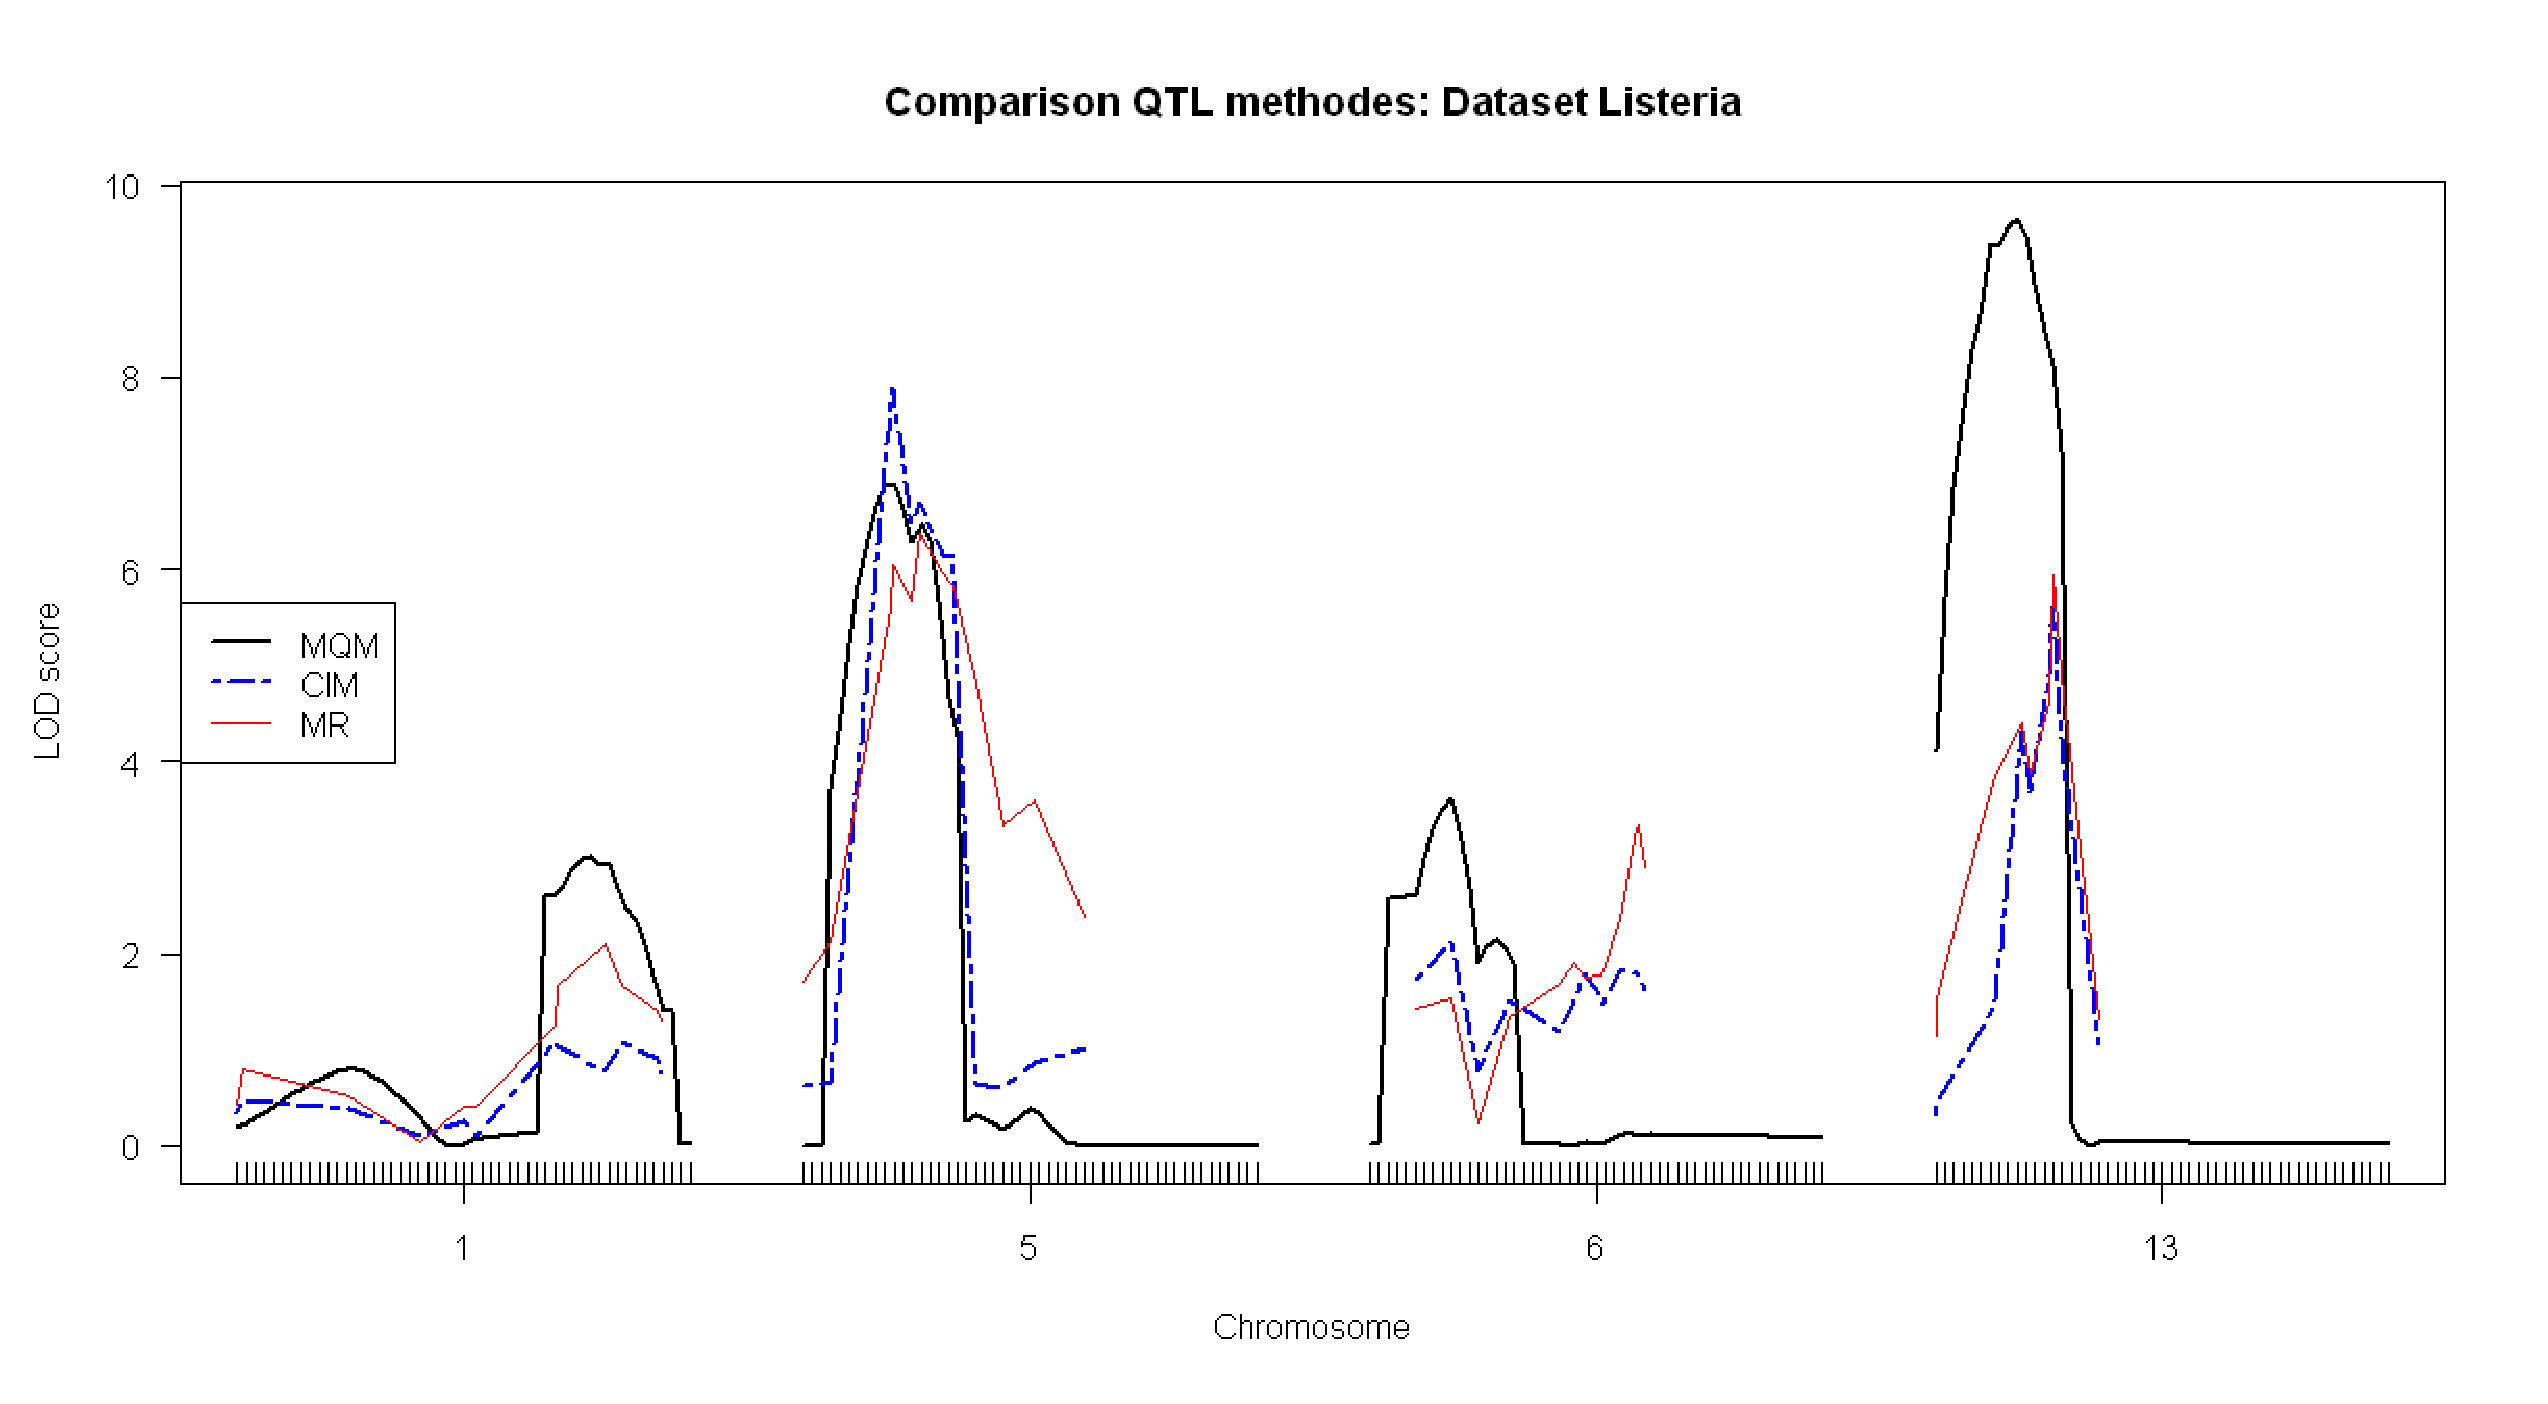
\includegraphics[height=8.0cm,width=12.0cm]{Images/DatasetListeria.eps}}
	  \label{fig:FigureListeria}
	  \caption{MQM in comparison with other QTLmapping methods (CIM, MR) using the dataset: \"listeria\". Using MQM we set cofactors every even marker, and do backward selection using a windowsize of 15 Cm. CIM also uses a window of 15Cm}
	\end{figure}
	
	\begin{figure}[ht]
	  \hfill
	  \fbox{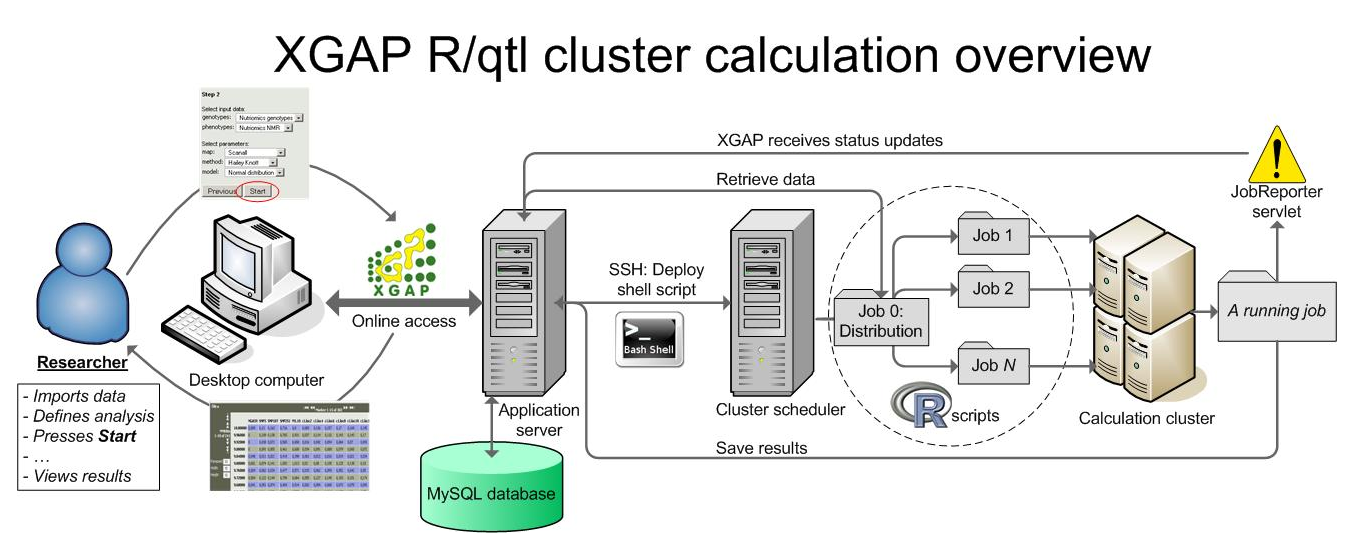
\includegraphics[height=6.0cm,width=12.0cm]{Images/Cluster_Layout.eps}}
	  \label{fig:FigureCluster}
	  \caption{Clusterlayout used at GBIC to do HPC analysis of QTLs using an opteroncluster controlled from the webinterface of a molgenis databaseserver}
	\end{figure}
	
	\begin{figure}[ht]
	  \hfill
	  \fbox{\includegraphics[height=6.0cm,width=12.0cm]{Images/taskviewer.eps}}
	  \label{fig:FigureTaskman}
	  \caption{Overview of the tasmanager plugin. Seen here are different tasks that have been submitted to the cluster. For an overview of the statuscolors see table \ref{tbl:tabelSTATUS}}
	\end{figure}
\end{document}
